\documentclass{article}
\usepackage{amsmath}
\usepackage{nips15submit_e,times}
\usepackage{amsfonts}
\usepackage{algorithm}
\usepackage{algorithmicx}
\usepackage{algpseudocode}
\usepackage{booktabs}
\usepackage{graphicx}
\usepackage{subfigure}
\usepackage{placeins}

\title{Logistic Regression and Softmax Regression for Emotion recognition}

\setlength\parindent{0pt}
\begin{document}
\maketitle

\begin{abstract}
In this report, we implemented logistic regression and softmax regression to complete emotion recognition task with CAFE dataset. PCA was trained using the training set and then the hold out and test set were projected to low dimensional distribution using the eigenvector generated by PCA. We implemented logistic regression via batch gradient descent for distinguish "happy" faces and "maudlin" ones and achieved an average accuracy of 90\% (0.21) and the average accuracy for "anger" and "surprising" faces are 100\% (0.0).  We also compared different dimensions for choosing the parameter for PCA and fine tuned different learning rate for the updaing rule.
In addition, we implemented a multi-classifier based on softmax regression. The batch gradient descent was first applied and the average accuracy is 82\% (0.12) on multiple emotion recognition problem.
Besides, the stochastic gradient descent was compared with the batch version and it was verified that stochastic version is faster than the batch version.  Through producing the confusion matrix of the model, we found the most frequently mistake is to classify "maudlin" as "surprising". The weights were also visualized and looked like faces in different emotions, which was explained from the aspect of magnifying significant signal. In the last, we trained our softmax regression model for face recognition and the average accuracy is 95\%(0.01).

\end{abstract}

\section{Load and preprocess the data}

\subsection{Introduction}
In this project, our task is to complete emotion identification. The dataset used is California Facial Expressions (CAFE). For this dataset, there're 10 identities corresponding to 8 different kinds of emotions("happy","happy with teeth","maudlin","surprise","fear","anger","disgust", "neutral") for each subject. The instruction of assignment orders us to choose one kind of happy between "happy" and "happy with teeth" and overlook the neural faces. Therefore, the final dataset should be 10 subjects and 6 emotions for each person. Figure \ref{figure: sixemotion} displays six different emotions.
\begin{figure}[ht]
\begin{center}
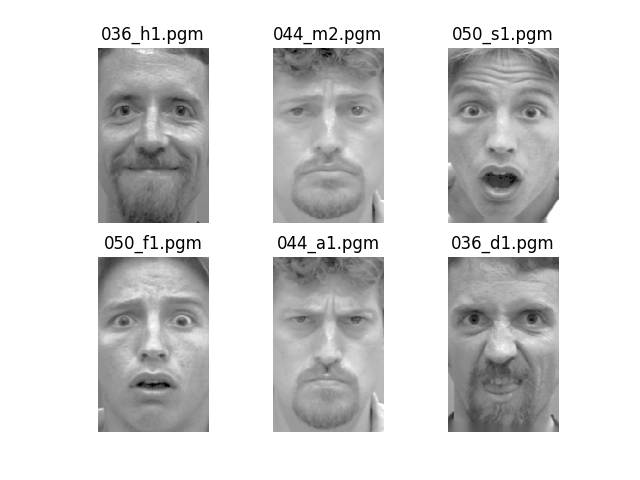
\includegraphics[scale=0.5]{images/six_face.png}
\end{center}
\caption{Samples of 6 emotions in CAFE Dataset}
\label{figure: sixemotion}
\end{figure}
After deleting both "happy with teeth" and "neural", the size of dataset should be $10\times6=60$. Besides, the size for each image is $380\times240$ and in order to consider it as one item of data, it was reshaped into size $380 \times 240 = 91200$, which is a row vector.
\paragraph{PCA} By reshaping one data into a row vector, each row can be considered as one piece of data with $91200$ dimensions. It is obvious that the dimension is too high to use in the following classification model. Therefore, Principal Components Analysis was introduced, which can be utilized to reduce the dimension of dataset.

\subsection{Methods}
As mentioned in subsection 1.1, PCA was introduced into reducing the dimension of data, therefore, we are going to introduce how to apply PCA in our project. The following Table shows the rough algorithm of PCA.
\begin{algorithm}
        \caption{Principal Components Analysis (Original Version)}
        \begin{algorithmic}[1]
            \Require original data (Shape: $N\times Old \;Dimension$)
            \Ensure  projected data (Shape: $N\times New \;Dimension$)
             \State standardize input data to 0-mean and 1-std
             \State calculate covariance matrix by $A^TA$
             \State calculate eigenvector and eigenvalues of $A^TA$
             \State choose top-k eigenvectors as the projection matrix
             \State project the standardized data with the projections matrix
        \end{algorithmic}
\end{algorithm}
\par
However, when processing the eigenvectors and eigenvalues of the covariance matrix in step (3), the program encountered with a memory error. The reason that leads to the issue is the extemely high dimension. To be specific, the size of input for PCA should be $N\times 91200$ in our case, where N is the number of images. Therefore, the size of covariance matrix will be $91200\times 91200$ which is too large to calculate its eigenvectors and corresponding eigen values.
\par
An alternative method is to calculate the eigenvectors of $C = A^TA$ by calculating the ones of $AA^T$ at first. The process can be proved as equation (\ref{eigenvalue})
\begin{equation}
    \begin{split}
    AA^Tv_i &= \mu_iv_i\\
    \Rightarrow A^TAA^Tv_i &= A^T\mu_iv_i\\
    \Rightarrow A^TAA^Tv_i &= \mu_iA^Tv_i\\
    \Rightarrow C(A^Tv_i)  &= \mu_i(A^Tv_i)\\
    \label{eigenvalue}
    \end{split}
\end{equation}
Therefore, it it obvious to find that the eigenvector of the original covariance matrix is $A^Tv_i$. Simultaneously, the eigenvalues are the same as matrix $AA^T$. According to the above process, we change the original method a little as Algorithm 2. It should be noted that the goal of step (5) is to transform each eigenvector to be unit vector.
\begin{algorithm}
        \caption{Principal Components Analysis (Modified Version)}
        \begin{algorithmic}[1]
            \Require original data (Shape: $N\times D$), k: dimension to choose
            \Ensure  projected data (Shape: $N\times k$)
             \State subtract the mean image from original data
             \State calculate covariance matrix by $\frac{1}{N}AA^T$
             \State calculate eigenvectors $v$ and eigenvalues of $\frac{1}{N}AA^T$
             \State calculate true eigenvector for $\frac{1}{N}AA^T$ by $\frac{1}{N}A^Tv$
             \State scale the eigenvectors by dividing $\sqrt{N\times eigenvalues}$
             \State choose top-$k$ eigenvectors as the projection matrix
             \State project the standardized data with the projections matrix
        \end{algorithmic}
\end{algorithm}
\par

\subsection{Results}
6 eigenfaces are shown in Figure \ref{figure: eigenfaces}. Eigenfaces are generated by reshaping the eigenvectors the same shape as the original image.
\begin{figure}[ht]
\begin{center}
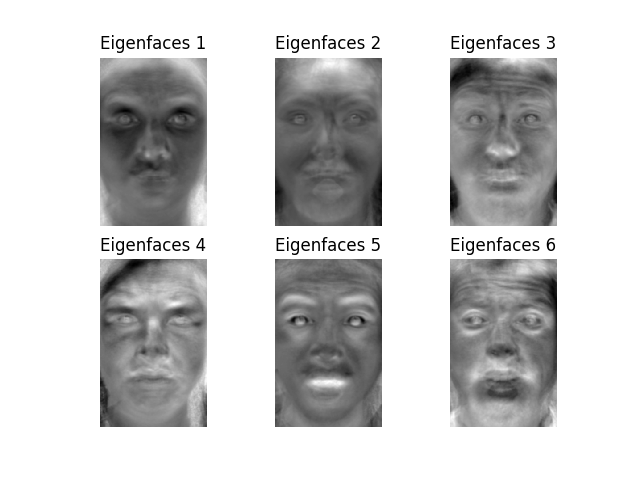
\includegraphics[scale=0.5]{images/eigenfaces.png}
\end{center}
\caption{6 eigenfaces formed by eigenvectors}
\label{figure: eigenfaces}
\end{figure}
\paragraph{Sanity check for PCA} There is a simple way to check whether our pca algorithm was implemented correctly. Suppose projecting $M$ images to the low dimension using eigenvector, it will get a bunch of scalars whose average is 0, and whose standard deviation is $\lambda^{0.5}$. By testing by this criteria, our pca is implemented correctly.
\subsection{Discussion}
\paragraph{For question: why is it important to only use the training data to compute the principle components?
}
PCA is a dimensionality reduction technique which finds "important directions" (basis vectors which capture most variation of the data) inherent in the dataset. It projects data points into these basis vectors to obtain a low dimensional representation of the data points. Now, if you use test data also to find these basis vectors, and then project training data over these vectors and learn some classifier, you'll be using test data also to learn a representation for the training data, which is not the common practice. Also, such an approach won't have any real world application (unless you use Online PCA and some semisupervised online classifier)as in real world application you won't have test data beforehand.

\section{Logistic Regression}

\subsection{Introduction}

Logistic regression can be conceptualized as a single neuron training in a batch of $d$-dimensional inputs vector $x\in \mathbb{R}^{d}$ and producing an output $y$ between $0$ and $1$ which is the probability that the input belongs to some categories.

The output of $y$ is parameterized by $w$:
\begin{align}
    y = P(C_{1}|x) &= \frac{1}{1+e^{-w^{\top}}x} = \sigma(w^{\top}x) \\
    P(C_{0}|x) &= 1 - P(C_{1}|x) = 1 - y \\
    \sigma(z) &= \frac{1}{1+e^{-z}}
\end{align}

where $\sigma$ is $sigmoid$ activation function used in this assignment. The cross-entropy cost function is defined as following which is the loss function we will minimize over training data to update weights $w$:
\begin{align}
    E(w) = -\sum_{n=1}^{N}\{t^{n}ln(\sigma(y^{n}))+(1-t^{n})ln(1-\sigma(y^{n}))\}
\end{align}

We use average loss reporting results:
\begin{align}
    E(w) = -\frac{1}{N}\sum_{n=1}^{N}\{t^{n}ln(\sigma(y^{n}))+(1-t^{n})ln(1-\sigma(y^{n}))\}
    \label{equation: loss_lr}
\end{align}

Here, $t^{n}\in \{0,1\}$ is the true label of $n$th sample and $y^{n}$ is the output value produced by model therefore $\sigma(y^{n})\in \{0,1\}$ represent the probability of $x^{n}$ that is classified as some categories.

We minimize cost function as in equation (\ref{equation: lr_gradient}) via gradient descent to update parameters $w$ during training phase, the derivative of $E(w)$ with respect to $w$ is:
\begin{align}
    -\frac{\partial E(w)}{\partial w} = \sum_{n=1}^{N}(t^{n}-\sigma(y^{n}))x^{n}
    \label{equation: lr_gradient}
\end{align}

\subsection{Methods}

The problem we work on Logistic Regression basically consists of two parts which are the evaluation on Happy vs Maudlin training set and on Afraid vs Surprised training set respectively.

\subsubsection{Batch Gradient Descent}

We minimize the cost function as in equation (\ref{equation: loss_lr}) to update parameters $w$ and we repeat implementing batch gradient descent 10 times and 10 epochs each time.

\begin{algorithm}
  \caption{Batch Gradient Descent}
  \begin{algorithmic}[1]
    \State initialize $w\leftarrow$ random value
    \For{$ t = 0,\cdots,10$}
      \State split dataset into training/holdout/test set
      \For{$i = 0,\cdots,10$}
        \State $w(i+1)=w(i)-\alpha \sum_{n=1}^{N}\nabla E^{n}(w)$
      \EndFor
    \EndFor
  \end{algorithmic}
\end{algorithm}

\subsubsection{Training}

The input $x$ is encoded as a matrix with $\mathbb{R}^{n\times d}$ dimension where $n$ is the number of images and $d$ is the number of image features and the label $y$ is encoded as $0$ or $1$ with $\mathbb{R}^{n\times 1}$ dimension representing Maudlin or Happy respectively.

We try three different learning rates: $0.3$ that is too high, $0.001$ that is too small and $0.01$ that is just right $1$ time on $10$ epochs. We also repeat implementing gradient descent $10$ times, pick each subject as the test set each time and randomly pick a subject to be the holdout set, the subject used as test set is exclusive and will not be used as holdout set and training set.

To avoid over-fitting, early stoping can be used on training based on holdout set error. Hence there is a little tricky way: we save the best weights any time holdout set loss is less than it has been before. For testing part, use best weights to evaluate test set and report results.

\subsection{Result}

Figure 1 shows the training loss and holdout loss averaged over 10 runs along with the standard deviation for 2,4,8 and 10 epochs on $10$ principle components using $0.01$ learning rate. It can be seen from Fig.1 that the overall tendency of train loss and holdout loss are decreasing and do not go up at some epochs. The model converged around epoch $6th$ to its optimals.

\begin{figure}
\begin{center}
\begin{minipage}[t]{0.4\linewidth}
  \centering
  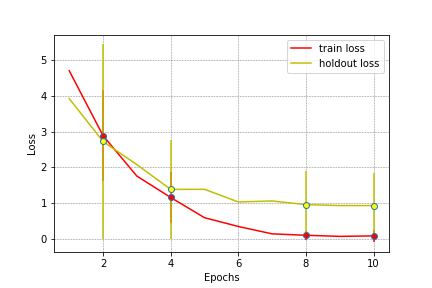
\includegraphics[width=2.5in]{images/hm_loss_recog_85acc.png}
\end{minipage}
\begin{minipage}[t]{0.5\linewidth}
  \centering
  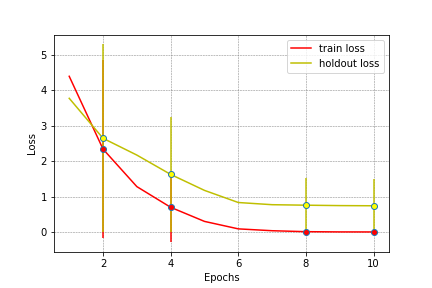
\includegraphics[width=2.5in]{images/as_loss_recog_100acc.png}
\end{minipage}
\caption{Train loss and holdout loss averaged over 10 runs along with standard deviation for 2,4,8 and 10 epochs. Note that $0.01$ learning rate and $10$ principle components are used during training phase. \textbf{Left:} training loss and holdout loss along with standard deviation on \textbf{Happy vs Maudlin}. \textbf{Right:} training loss and holdout loss along with standard deviation on \textbf{Anger vs Surprised}.}
\end{center}
\end{figure}

Table 1 shows the average accuracy over the 10 runs and 10 epochs per run with standard deviation in parentheses on $10$-dimensional input features (dimensionality reduced by PCA). It can be seen from the table that both average accuracy on Happy vs Maudlin and Anger vs Surprised dataset increase when using larger $k$ and reache 100\% with 0 standard deviation because with the increasement of $k$, the model can learn more features to distinguish one class from another and the scale of the dataset is too small (overall 20 images) that only 2 images are used as test set to evaluate the model.

\begin{table}
\begin{center}
\setlength{\tabcolsep}{9mm}
\begin{tabular}{c|cc}
\toprule
Experiment& Happy vs Maudlin & Anger vs Surprised \\
\midrule
LG + BGD k = 2 & 60.0 \% (0.21) & 60.0 \% (0.21) \\
\midrule
LG + BGD k = 4 & 60.0 \% (0.21) & 90.0 \% (0.21) \\
\midrule
LG + BGD k = 8 & 75.0 \% (0.26) & 95.0 \% (0.16) \\
\midrule
LG + BGD k = 10 & 90.0 \% (0.21) & 100.0 \% (0.0) \\
\bottomrule
\end{tabular}
\caption{Average accuracy and standard deviation in parentheses over 10 runs with 10 epochs per run in Happy vs Maudlin and Anger vs Surprised on top $k$ principle components using $0.01$ learning rate. Note that LG and BGD correspond to Logistic Regression via Batch Gradient Descent.}
\end{center}
\end{table}

Figure 2 shows the training set error (cross-entropy loss) along with the standard deviation for 2,4,8 and 10 epochs on $10$ principle components for three different learning rates on Happy vs Maudlin and Anger vs Surprised. It can be seen from Fig.2 that train loss with learning rate $0.001$ which is too small decreases way smaller than learning rate $0.01$ that is just right and learning rate $0.3$ that is too high. Besides, model with learning rate that is too high results in overfitting and causes the dropping in accuracy although the loss decreases faster that one that is just right.

% hm_loss_recog_lr_45/0.16_90/0.21_75/0.26.png
% as_loss_recog_lr_55/0.28_100/0.0_90/0.21.png
\begin{figure}
\begin{center}
\begin{minipage}[t]{0.4\linewidth}
  \centering
  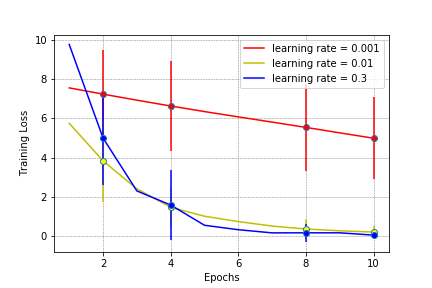
\includegraphics[width=2.5in]{images/hm_loss_lr.png}
\end{minipage}
\begin{minipage}[t]{0.5\linewidth}
  \centering
  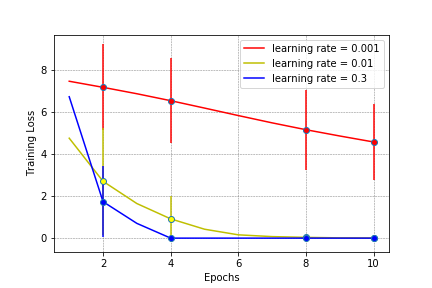
\includegraphics[width=2.5in]{images/as_loss_lr.png}
\end{minipage}
\caption{Train loss for the three different learning rates along with the standard deviation for 2,4,8 and 10 epochs on $10$ principle components. \textbf{Left:} train loss along with standard deviation on \textbf{Happy vs Maudlin}. Learning rate 0.001 (too small) with average accuracy and standard deviation $45\%(0.16)$, learning rate 0.01 (best) with average accuracy and standard deviation $90\%(0.21)$ and learning rate 0.3 (too high) with average accuracy and standard deviation $75\%(0.26)$. \textbf{Right:} train loss along with standard deviation on \textbf{Anger vs Surprised}. Learning rate 0.001 (too small) with average accuracy and standard deviation $55\%(0.28)$, learning rate 0.01 (best) with average accuracy and standard deviation $100\%(0.0)$ and learning rate 0.3 (too high) with average accuracy and standard deviation $90\%(0.21)$.}
\end{center}
\end{figure}

\subsection{Discussion}

For problem \textbf{Think about why we only need one logistic output unit if we’re classifying two classes?} One logistic output unit can output 0 and 1 to denote two classes.

For problem \textbf{How does this differ from what we observed above? Why do you think that it?} The logistic regression performs better on Anger vs Surprised than Happy vs Maudlin. We suggest that the reason performance differs between Anger vs Surprised and Happy vs Maudlin is that the facial expression changing from Anger to Surprised is much more apparent than that from Happy to Maudlin. We looked into Happy vs Maudlin and Anger vs Surprised dataset finding that happy face looks similar to sad face although it is happy and maudlin. While anger face is quite different from surprise face as the open mouth.

\section{Implement Softmax Regression via Gradient Descent}

\subsection{Introduction}
Section 2 talks about logistic regression, which basically is a binary classifier, whereas softmax regression a multi-class classifier. Given an input $x_n$, the output of softmax regression can be denoted as equation (\ref{equation:an}) and (\ref{equation:yn}).
\begin{equation}
\begin{split}
a_k^n = w_k^T x^n
\end{split}
\label{equation:an}
\end{equation}

\begin{equation}
\begin{split}
    y_n = \frac{exp(a_k^n)}{\sum_{k^{'}}{exp(a_{k^{'}}^n)}}
\end{split}
\label{equation:yn}
\end{equation}
A more general way to define the cross-entrophy loss in multi-class classifier, it should be like equation (\ref{equation:multiloss}) in the following.
\begin{equation}
E = -\sum_n\sum_{k=1}^{c}t_k^n ln{y_k^n}
\label{equation:multiloss}
\end{equation}
Besides, in order to eliminate the influence of number of data, the loss function in equation(\ref{equation:multiloss}) should be averaged over the number of data as equation (\ref{equation:multiloss2}).
\begin{equation}
    \begin{split}
    E = -\frac{1}{N}\sum_{n=1}^N\sum_{k=1}^{c}t_k^n ln{y_k^n}
    \end{split}
    \label{equation:multiloss2}
\end{equation}
What should be noted in multi-classifier is the ground-truth of the data. Instead of using the class id(e.g. 0,1,2...) as $Y$ directly, it should use one-hot encoding. For example, if one piece of data belongs to class 2, the authentic $Y$ should be $[0,0,1,0,0,0]$ in a task with 6 classes.
\subsection{Methods}
\subsubsection{Gradient Calculation}
Given the loss function like equation (\ref{equation:multiloss2}), it is still necessary to use gradient descent to find the corresponding weights locating at the minimum. Therefore, we should also to compute the derivative with respect to each weight at each updating moment. First of all, the gradient of equation (\ref{equation:multiloss2}) with respect to $w_{jk}$ can be derived as equation (\ref{equation:gradient})
\begin{equation}
-\frac{\partial E^n(w)}{\partial w_{jk}}= \sum_{k'} -\frac{\partial E^n(w)}{\partial y_{k'}^n}\cdot \frac{\partial y_{k'}^n}{\partial a_k^n}\cdot \frac{a_k^n}{w_{jk}}
\label{equation:gradient}
\end{equation}
Further, the first term of RHS can be deduced into
$$-\frac{\partial E^n(w)}{\partial y_{k'}^n}= \frac{t_{k'}^n}{y_{k'}^n}$$
While for the second fraction term, it should be considered with two cases. Te First one is when $k'=k$
\begin{equation}
\begin{split}
     \frac{\partial y_{k'}^n}{\partial a_k^n}
     &=\frac{\exp(a_{k'}^n) \sum_{k'} \exp(a_{k'}^n)-\exp(a_{k'}^n)exp(a_k^n)}{(\sum_{k'}\exp(a_{k'}^n))^2}\\
     &= \frac{\exp(a_{k'}^n)(\sum_{k'}\exp(a_{k'}^n)-\exp(a_k^n))}{(\sum_{k'}\exp(a_{k'}^n))^2}\\
     &= y_{k'}^n(1-y_k^n)
\end{split}
\end{equation}
And the second case is when $k'\neq k$
\begin{equation}
    \begin{split}
    \frac{\partial y_{k'}^n}{\partial a_k^n}=\frac{0-\exp(a_k^n)\cdot \ exp(a_{k'}^n)}{(\sum_{k'}\exp(a_{k'}^n))^2}= -y_k^n\cdot y_{k'}^n \\
    \end{split}
\end{equation}
Then the two cases can be merged with the following format
\begin{align*}
\frac{\partial y_{k'}^n}{\partial a_k^n} = y_{k'}^n\cdot \delta_{kk'}-y_{k'}^ny_k^n\\
\end{align*}
Finally, the last term is
\begin{equation}
\frac{\partial a_k^n}{\partial w_{jk}} = x_j^n
\end{equation}
Thus,
\begin{equation}
\begin{split}
 -\frac{\partial E^n(w)}{\partial w_{jk}}&=x_j^n \sum\limits_{k'}^C{\frac{t_{k'}^n}{y_{k'}^n}}\cdot (y_{k'}^n\cdot \delta_{kk'}-y_{k'}^ny_k^n)\\
 &= x_j^n(\sum\limits_{k'}^C{t_{k'}^n}\delta_{kk'}-\sum\limits_{k'}^C {t_{k'}^n}y_{k}^n)
 \text{, where} \sum\limits_{k'}^C {t_{k'}^n} =1\\
    &= x_j^n(t_k^n - y_k^n)
\end{split}
\end{equation}
\subsubsection{Stochastic Gradient Descent}
Instead of using only batch gradient descent, for the experiment of softmax regression, we use another mode of gradient descent called stochastic gradient descent. The difference between the batch mode and stochastic mode is that weights are updated for each sample and the samples are shuffled randomly. The algorithm is displayed in the following.
\begin{algorithm}
        \caption{Stochastic Gradient Descent}
        \begin{algorithmic}[1]
             \State $w\leftarrow0$
             \For{$t = 0 \to T^{'}$}
                \State shuffle the training set
                \For{$n = 1 \to N$}
                    \State $w(t+1) = w(t) -\alpha \nabla E^{n}(w)$
                \EndFor
             \EndFor
        \end{algorithmic}
\end{algorithm}
\subsubsection{Category Selection}
As mentioned above, "happy with teeth" were not included in our dataset. The reason is that the dataset will be balanced in this way. To be specific, if included all the happy faces, there will be 12 images for each identity for happy class whereas there will be 6 images for other classes. Intuitively, the model will learn more on happy but less on other emotions, which seems to be "unfair". Therefore, we only use 6 of happy faces in this project.
\subsection{Result}
\subsubsection{Evalution on all emotions via BGD}
Figure \ref{figure: loss_bgd} shows the variance of loss on training set and on hold-out set.
\begin{figure}[ht]
\begin{center}
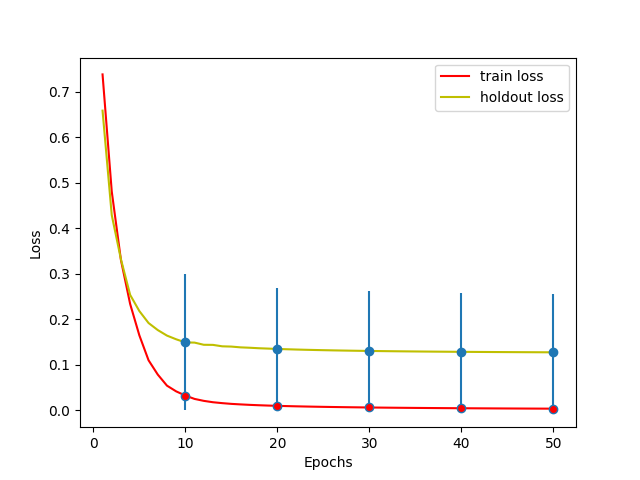
\includegraphics[scale=0.5]{images/softmax_bgd.png}
\end{center}
\caption{Train loss and holdout loss with standard deviation on epoch 10,20,30,40,50}
\label{figure: loss_bgd}
\end{figure}
From Figure \ref{figure: loss_bgd}, the first discovery is that there exist a distinct local minimum in hold-out curve. It can be explained by the theory that when the number of epoch goes up, the model will experience from "stupid" to "overfit". Therefore, approximately, epoch 10 is the best model during the above training process.
\par
In addition, when observing the standard deviation on both on training set and hold-out set, we can find that the standard deviation on training set is relatively small, whereas the ones on hold-out set is large. The reason is that we only have 6 images (1 identity) as hold-out set.
\par
 The result of softmax regression for 6 emotions and its parameters are displayed in the Table \ref{table: softmax_bgd}. Besides, we set the demension of PCA to $10,20,40$ and found when dimension goes up, the accuracy becomes higher, which can be explained by more dimensions contain more information for each data.
\begin{table}
  \setlength{\tabcolsep}{9mm}
  \label{table: softmax_bgd}
  \centering
  \begin{tabular}{c|c|c|c}
    \toprule
    \cmidrule(r){1-4}
    Times     &Accuracy&Learning rate&dimensions \\
    \midrule
    10  &71\% (0.12)&0.05&10\\
    10  &76\% (0.11)&0.05&20\\
    10  &82\% (0.12)&0.05&40\\
    \bottomrule
  \end{tabular}
  \caption{Different accuracy and standard deviation under diffferent dimensions}
\end{table}
\par
In terms of the best model we created the confusion matrix on the test set. Confusion matrix is a table that is used to measure the performance of a classification model on a set of test data. Each entry $C_{ij}$ represents when the image is classified as class $j$ whereas the true label is class $i$. Therefore, the closer the entries on main diagonal is to 100\%, the better the model's performance is. Figure \ref{figure: confusion_bgd} shows the confusion matrix of model via batch gradient descent. We can find in most cases that the model performs excellent. However, the most evident wrong classification case is when true label is maudlin, it's likely to be classified as anger because these two emotions are indeed similar to each other.
\begin{figure}[ht]
\begin{center}
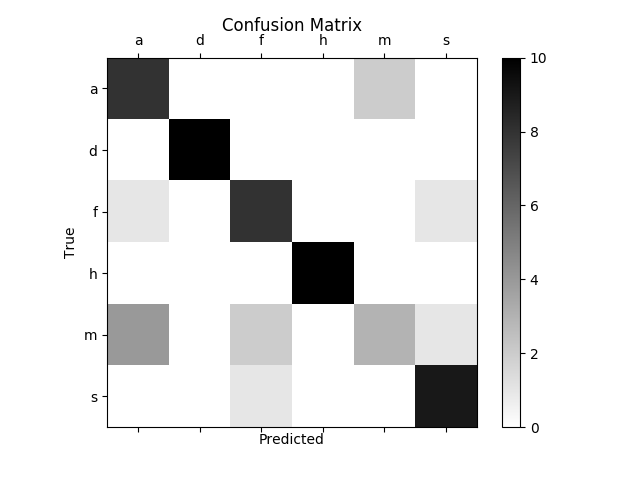
\includegraphics[scale=0.5]{images/confusion_bgd.png}
\end{center}
\caption{Confusion matrix on 6 emotions via batch gradient descent}
\label{figure: confusion_bgd}
\end{figure}
\subsubsection{Batch versus stochastic gradient descent}
Figure \ref{figure: loss_sgd} shows that the best model exist at $\text{epoch}=6$ because after that the hold out loss becomes nearly constant.
\begin{figure}[ht]
\begin{center}
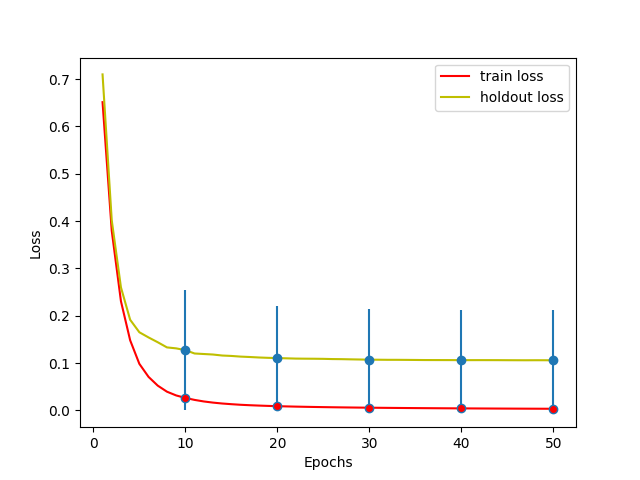
\includegraphics[scale=0.5]{images/softmax_sgd.png}
\end{center}
\caption{Train loss and holdout loss with standard deviation on epoch 10,20,30,40,50 based on stochastic gradient descent}
\label{figure: loss_sgd}
\end{figure}
\paragraph{Is stochastic gradient descent faster, in terms of minimizing the error
in fewer epochs? Explain your result}
Besides, Figure \ref{figure:bgd_sgd} shows the comparison between training loss based on BGD and SGD. It is obvious that the model converges to the local minimum quickly in stochastic version than the batch one. The reason leading to this can be find from the differences in Algorithm 1 and Algorithm 4. For batch version, the weights of model are updated for each epoch but for the stochastic version, the updating rule will iterate each data and update the weight during just one epoch. Therefore, in our project, if running with 50 epochs, the weights will be updated for $50$ times and be updated for $50\times N= 50N$ where $N$ is the number of training set.
\begin{figure}[ht]
\begin{center}
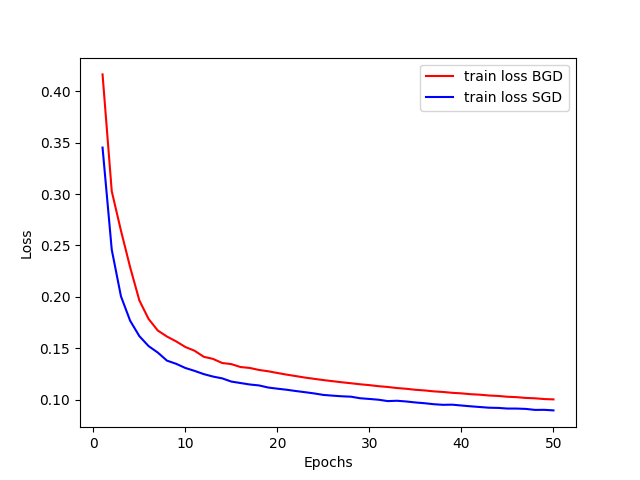
\includegraphics[scale=0.5]{images/bgd_sgd.png}
\end{center}
\caption{Training loss based on BGD and SGD}
\label{figure:bgd_sgd}
\end{figure}
\par Figure \ref{figure: confusion_sgd} displays the confusion matrix of softmax regression based on stochastic gradient descent. The result seems to be similar to the on based on batch gradient descent and the most frequently wrong classification is to predict the query with true label "surprising" as label "frightening".
\begin{figure}[ht]
\begin{center}
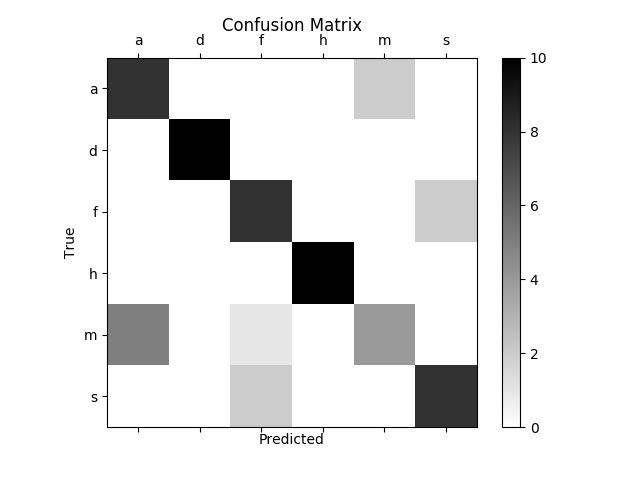
\includegraphics[scale=0.5]{images/confusion_sgd.png}
\end{center}
\caption{Confusion matrix on 6 emotions via stochastic gradient descent}
\label{figure: confusion_sgd}
\end{figure}
\subsubsection{Visualization of Weights}
In this subsection, we visualized the weights from the previous trained model. The method is to multiplied the trained weights separately $(w_1,w_2...,w_6)$ with the eigenvector, followed by reshaping the output vector into a image shape (e.g. $380\times 240$). The visualization images for each weight are shown in Figure \ref{figure: visualizaiton}.
\begin{figure}[ht]
\begin{center}
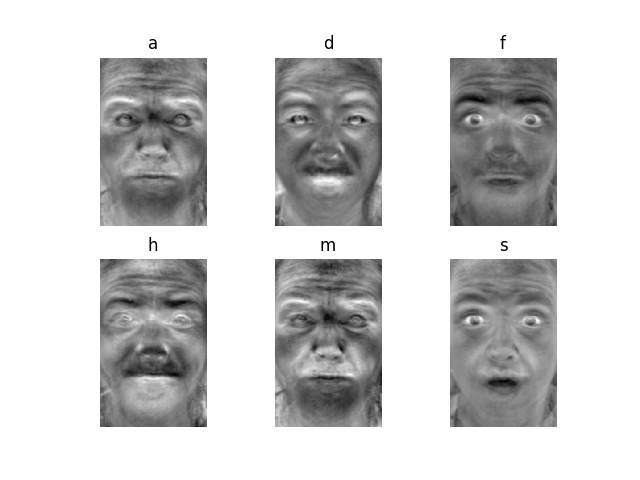
\includegraphics[scale=0.5]{images/visualization.png}
\end{center}
\caption{Visualizaiton of weights}
\label{figure: visualizaiton}
\end{figure}
From figure \ref{figure: visualizaiton}, we can see that they implies different emotions.
\paragraph{Explain why you end up seeing this. Include the six images in your report as a well-labeled figure.} For this question, I try to answer it from another aspect instead of mathematics. For each $w_i$, it should be in a shape of $1\times10$, where 10 is the dimension of each input data. And the 10 dimension are produced by PCA and the input is the image. Therefore, the 10 dimensions are related indirectly with the pixels, which can imply the location of the original image. And for $w_i$, it will magnify the signals of those pixels which should be included to play the role in classifying this image as class $i$. For example, for those pixels are important in "happiness", their corresponding $w_4$ will be larger. Because in our suppose, "happiness" is label 4. Therefore, $w_4$ looks like a ghost-like happy face.
\subsubsection{Face recognition}
We utilized softmax regression to classify the 10 subjects. To be specific, there are 10 subjects and for each person there will be 6 emotions. Therefore, in order to make the training set, hold out set and test set to be balanced. The above softmax process was executed for 6 times instead of 10 times and for each time, 10 subjects with the same emotions are selected to be set as the test set. The performance was shown in Table \ref{table: face_recog} and Figure \ref{figure: loss_recog} shows the loss curve over 50 epochs and Figure \ref{figure: visualization2} shows the 10 images reshaped by weights.

\begin{table}[ht]
  \setlength{\tabcolsep}{9mm}
  \label{table: face_recog}
  \centering
  \begin{tabular}{c|c|c|c}
    \toprule
    \cmidrule(r){1-4}
    Times     &Accuracy&Learning rate&dimensions \\
    \midrule
    6  &95\% (0.01)&0.05&40\\
    \bottomrule
  \end{tabular}
  \caption{Accuracy and standard deviation for face recognition}
\end{table}

\begin{figure}[ht]
\begin{center}
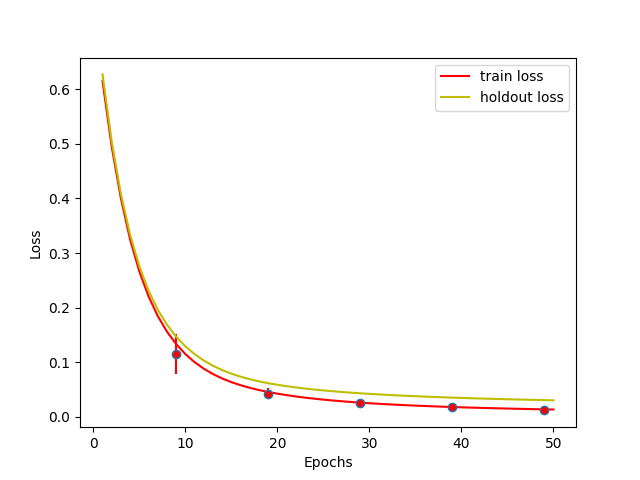
\includegraphics[scale=0.5]{images/loss_recog.png}
\end{center}
\caption{Face identification loss}
\label{figure: loss_recog}
\end{figure}

\begin{figure}[ht]
\begin{center}
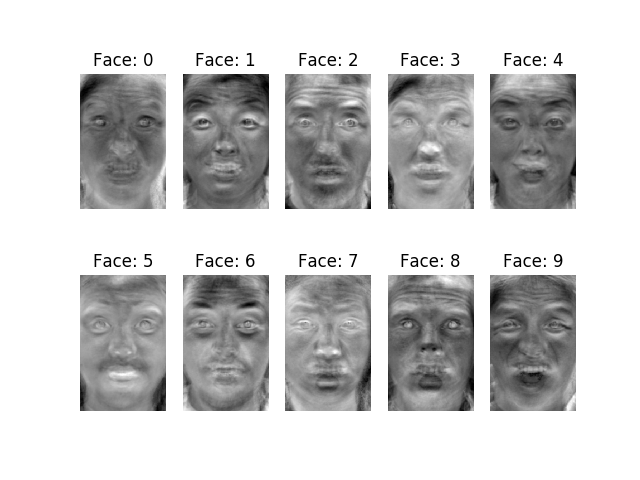
\includegraphics[scale=0.5]{images/visualization2.png}
\end{center}
\caption{Weights visualization of face recognition}
\label{figure: visualization2}
\end{figure}


\FloatBarrier

\section{Contribution}
We worked through all the problems together and discussed issues about how to implement and fine tune the models. Guanghao focused PCA algorithm and softmax regression part. Qimin focused on data preprocessing and logistic regression part. During writing the report, we respectively wrote the corresponding part and merged our report finally.
\end{document}
